%----------------------------------------------------------------------------
\chapter{Fejlesztőkörnyezet összeállítása}
%----------------------------------------------------------------------------

	OpenCL kód fejlesztése történhet Windows alatt NVIDIA Nsight Visual Studio
	Edition \cite{nsight} és Linux alatt GCC-vel \cite{gcc}.
	Az Open Source fejlesztőrendszer ingyenessége és az általa generált program hordozhatósága végett
	a Linux alatti fejlesztés mellett döntöttem. 
	Az OpenCL-t támogató hardverek legtöbbször CPU-k, GPU-k és az Intel MIC
	\cite{mic} kártyái.
	Ezekre való OpenCL kód fejlesztéséhez a gyártók biztosítanak Software Developement Kit-et (SDK).
	Ezek telepítése szinte bármelyik Linux disztribúción sikerülhet a megfelelő követelmények előzetes telepítése után.
	A Linux diszrók közül a CentOS-re \cite{centos} esett a választás, ami 
	csupán a fejlesztőkörnyezet egyszerűbb telepítése végett történt így.

\section{Software Developement Kit-ek (SDK) telepítése} \label{sect:sdk}
\subsection{nVidia támogatás telepítése}
	A legtöbb mai Linux disztrók tartalmaznak drivert az nVidia videó kártyákhoz.
	Ez az open source Nouveau, ami még nem támogatja az OpenCL-t.
	Így a hivatalos nVidia drivert fel kell telepítenünk.
	Ehhez először le kell tiltanunk a Nouveau betöltését.
	Ezt két helyen is meg kell tennünk: 
	egyrészt a \texttt{/etc/modprobe.d/blacklist.conf} fájlhoz hozzá kell adnunk a
	következő sort:
	\begin{lstlisting}
	blacklist nouveau
	\end{lstlisting}
	majd újragenerálni az INITial RAM File System-et (initramfs), ami a rendszer
	inicializásáért felelős:
	\begin{lstlisting}
	$ mv /boot/initramfs-$(uname -r).img /boot/initramfs-$(uname -r).img.bak
	$ dracut -v /boot/initramfs-$(uname -r).img $(uname -r)
	\end{lstlisting}
	másrészt a rendszer indító GRand Unified Bootloader-ben (GRUB) is le kell
	tiltani a betöltését a kernel opció alábbi paranccsal való kiegészítésével:
	\begin{lstlisting}
	nouveau.modeset=0
	\end{lstlisting}
	Továbbá a telepítéshez szükséges követelményeket a következő parancsokkal telepíthetjük:
	\begin{lstlisting}
	$ yum groupinstall "Development Tools"
	$ yum install kernel-devel kernel-headers dkms
	\end{lstlisting}
	Ekkor a rendszer újraindítása után készen állunk a hivatalos nVidia driver
	telepítésére. A drivert a következő linken lehet letölteni \cite{nvidia-driver}.
	A grafikus felületet a telepítés idejére le kell állítani az X grafikus
	kiszolgálót
	\begin{lstlisting}
	$ init 3
	\end{lstlisting}
	paranccsal, majd a konzolban telepíthető a driver, ami a legtöbb munkát elvégzi helyettünk. Ezután az
	\begin{lstlisting}
	$ init 5
	\end{lstlisting}
	paranccsal áttérhetünk a grafikus felületre, ahol a megfelelő környezeti változókat kiegészíthetjük.
	Legcélratörőbb, ha a \texttt{$\tilde{}$/.bashrc} fájlt módosítjuk és hozzáadjuk
	a következő sorokat:
	\begin{lstlisting}
	PATH=$PATH:$HOME/bin:/usr/local/cuda/bin
	export PATH
	
	CUDA_INSTALL_PATH=/usr/local/cuda
	export CUDA_INSTALL_PATH
	
	LD_LIBRARY_PATH=/usr/local/cuda/lib64:/opt/intel/opencl/bin
	export LD_LIBRARY_PATH
	
	NVSDKCOMPUTE_ROOT=/usr/local/cuda/lib64
	export NVSDKCOMPUTE_ROOT
	
	INTELOCLSDKROOT=/opt/intel/opencl
	export INTELOCLSDKROOT
	\end{lstlisting}
	Mivel az nVidia limitálja a kernel futási időt 5 másodpercben limitálja,
	hosszabb kernel futási idő esetén a rendszer lefagy.
	Ezt a korlátozást a \texttt{/etc/X11/xorg.conf} fájl \texttt{Device} részének a
	következővel való kiegészítésével érhetjük el:
	\begin{lstlisting}
	Option "Interactive" "boolean"
	\end{lstlisting}
	Érvényre juttatásához az X újraindítása szükséges (CTRL+ALT+Backspace).
	Ezután nagyobb problémák esetén már nem fogja lefagyasztani a rendszert a
	watchdog.

\subsection{Intel támogatás telepítése}
	A következő oldalról letölthetjük az SDK-t \cite{intel-sdk}.
	A kicsomagolás után az \texttt{./install-cpu.sh} program futtatásával
	telepíthető.
	Ezután még szükséges a \texttt{LD\_LIBRARY\_PATH} beállítása.

\subsection{Eclipse – Integrated Developement Environment}
	A fejlesztés és hibakeresés egy Integrated Developement Enviroment (IDE)
	segítségével könnyebb.
	Az open source Eclipse \cite{eclipse} fejlesztőkörnyezet a különböző pluginjaival épp
	megfelelő erre a célra.
	Például a C-nyelv fejlesztését segítő C/C++ Developement Tooling (CDT),
	a verziókövetést menedzselő EGit és a hibakeresést támogató GDT.
	A sok Eclipse változat közül az OpenCL fejlesztéshez legjobban az
	Eclipse for Parallel Application Developers verzió illik, mivel a korábban említett pluginokat már eleve tartalmazza.


\section{Új (Hello World) projekt létrehozása}
	Az OpenCL fejlesztését konyhanyelven bemutató OpenCL Programming Guide \cite{Munshi2011}
	könyvben szereplő Hello World programot a következő linken lehet letölteni
	\cite{hellow}.
	A kód fordítása elött egy Eclipse projektet létrehozunk és a
	fordításhoz szükséges beállításokat elvégezzük.

\subsection{Empty C project létrehozása}
	Először egy üres C projektet hozunk létre, ami folyamatát a \ref{fig:newproj} 
	ábrán látjuk. A korábban említettek szerint fordítónak a Linux GCC-t
	állítjuk be.
	\begin{figure}[H]
	\centering
	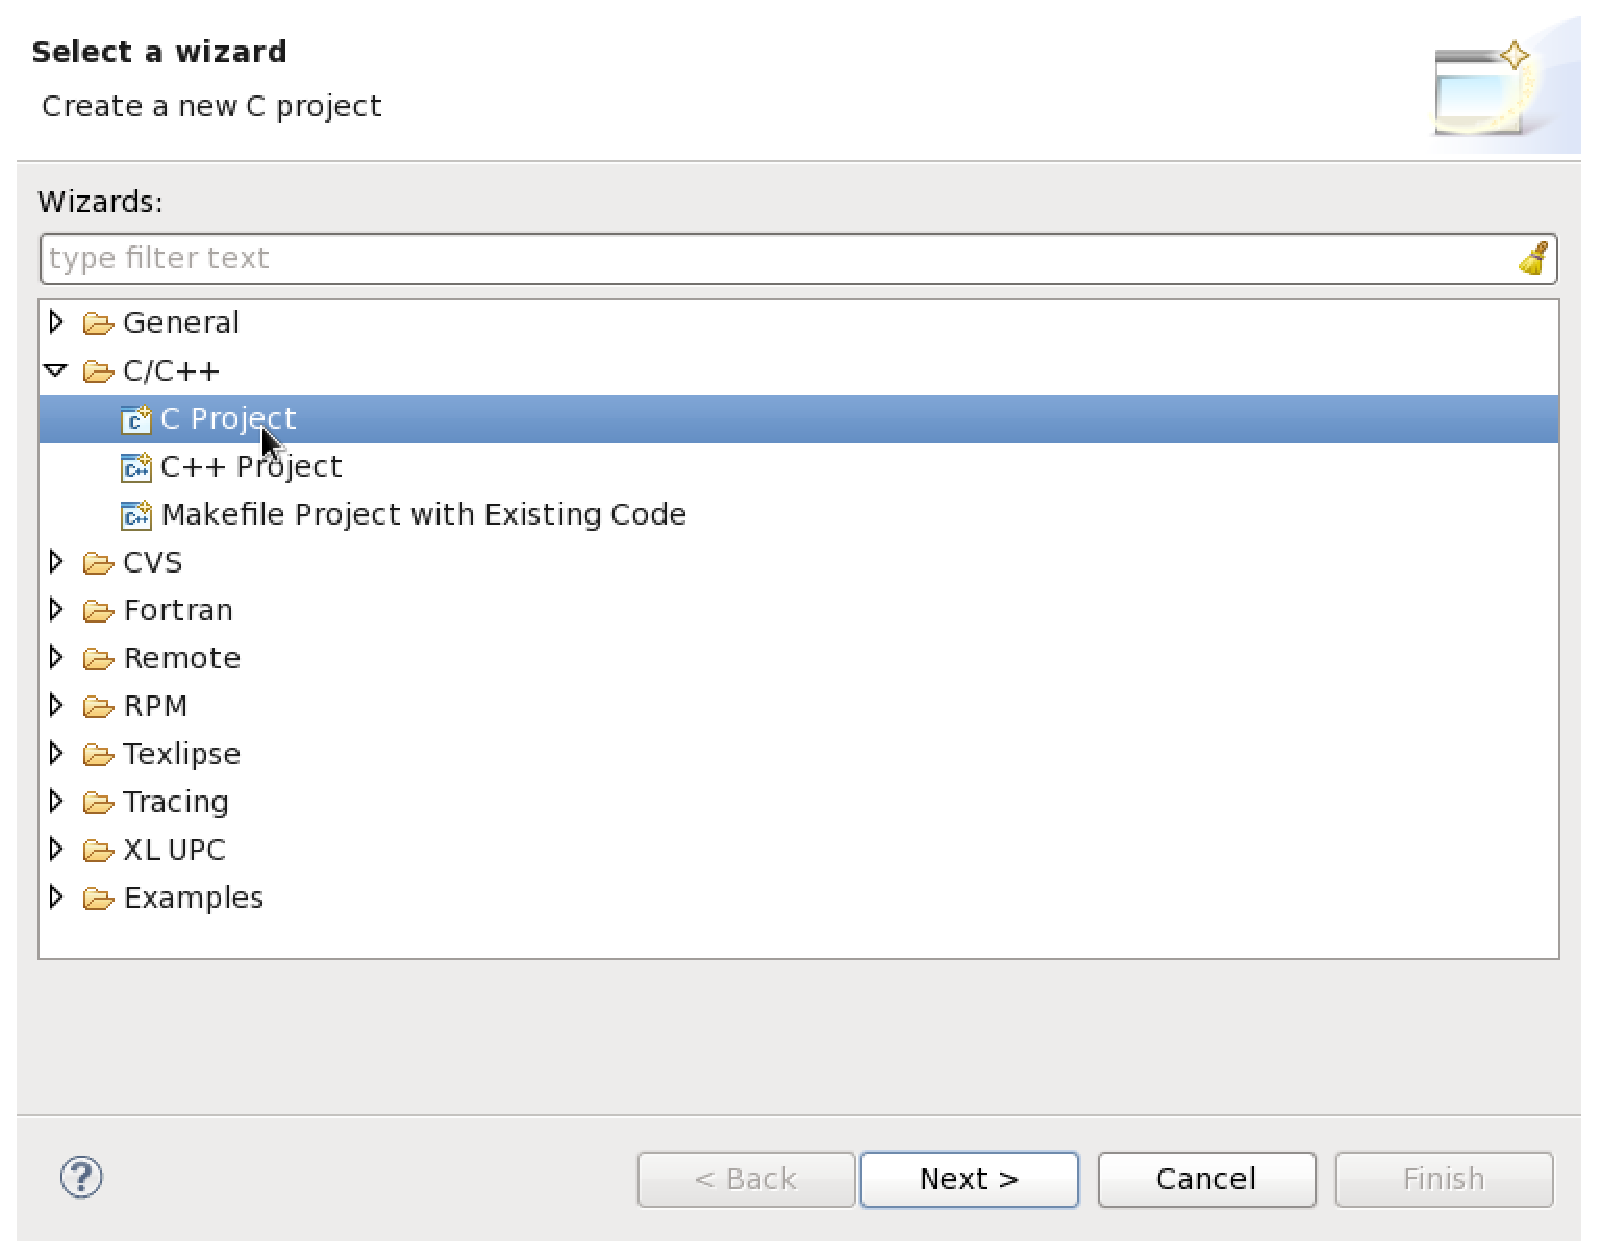
\includegraphics[width=67mm, keepaspectratio]{figures/eps/newC.eps}\hspace{1cm}
	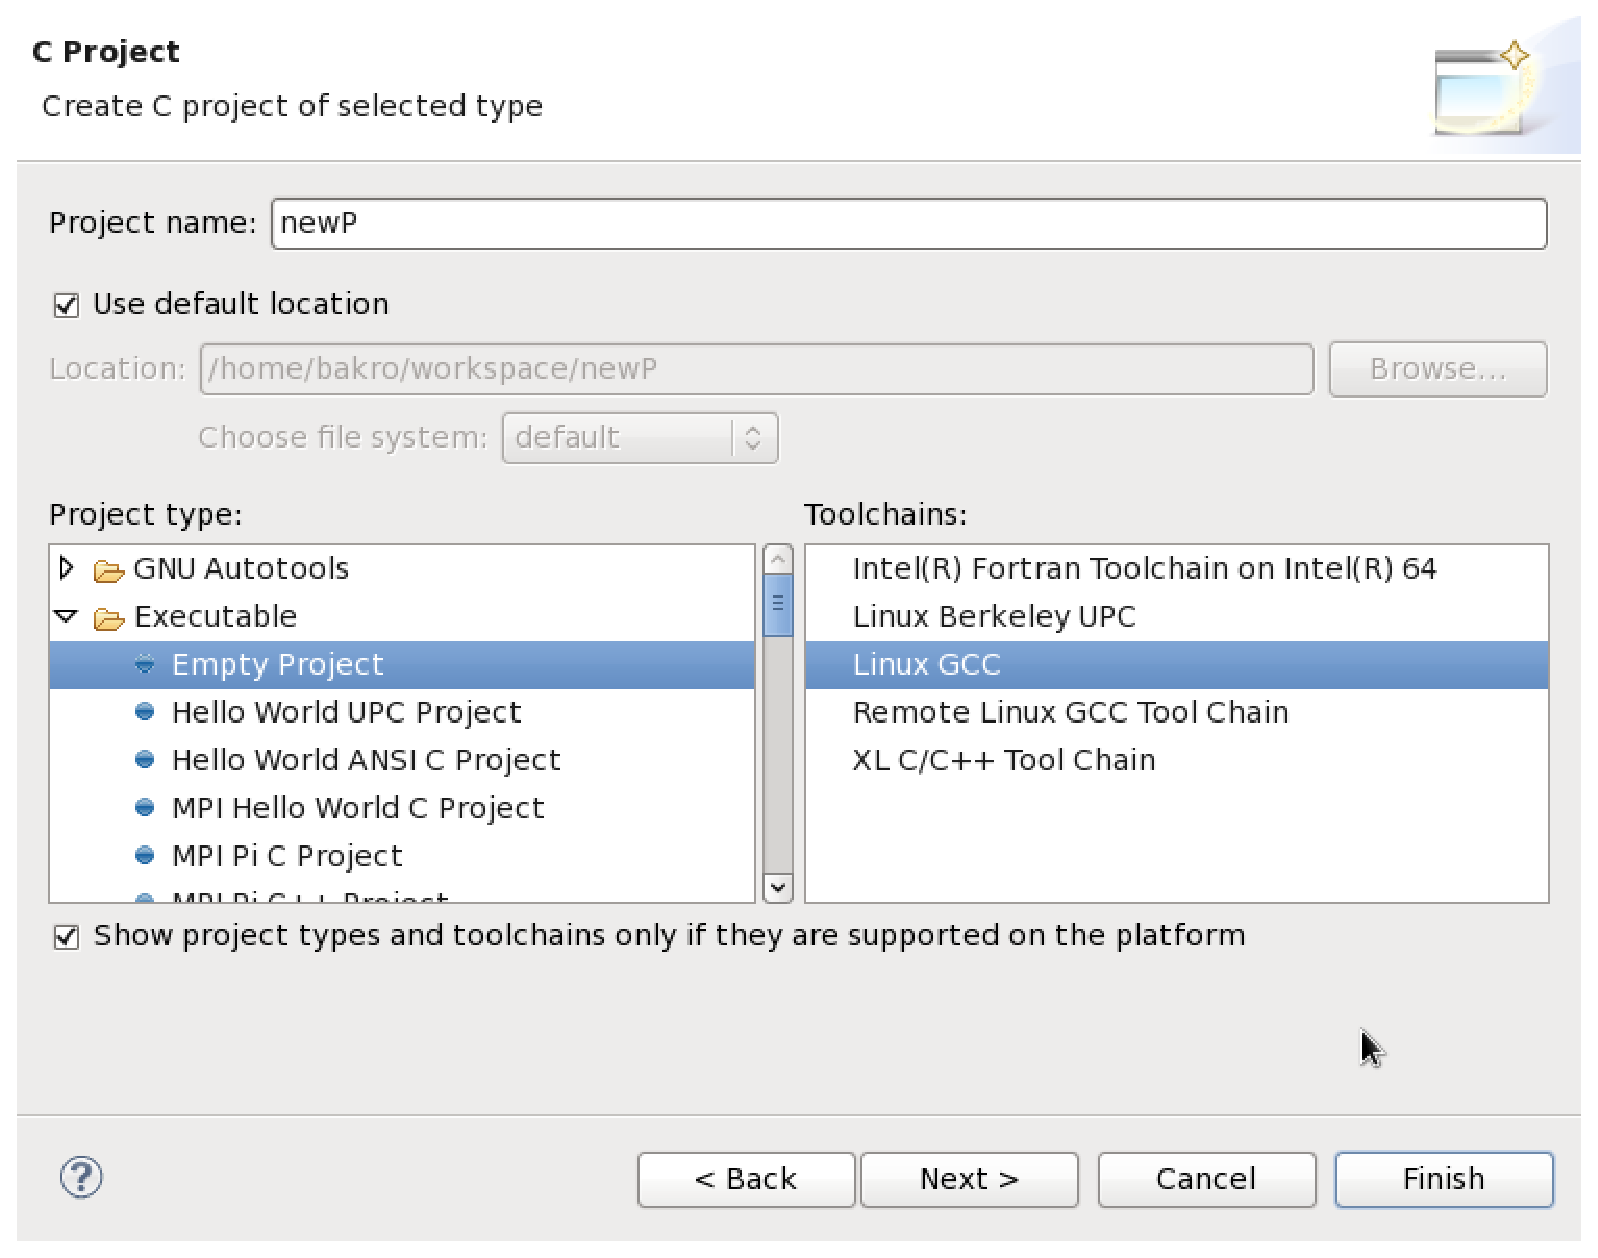
\includegraphics[width=67mm, keepaspectratio]{figures/eps/newP.eps}\\\vspace{5mm}
	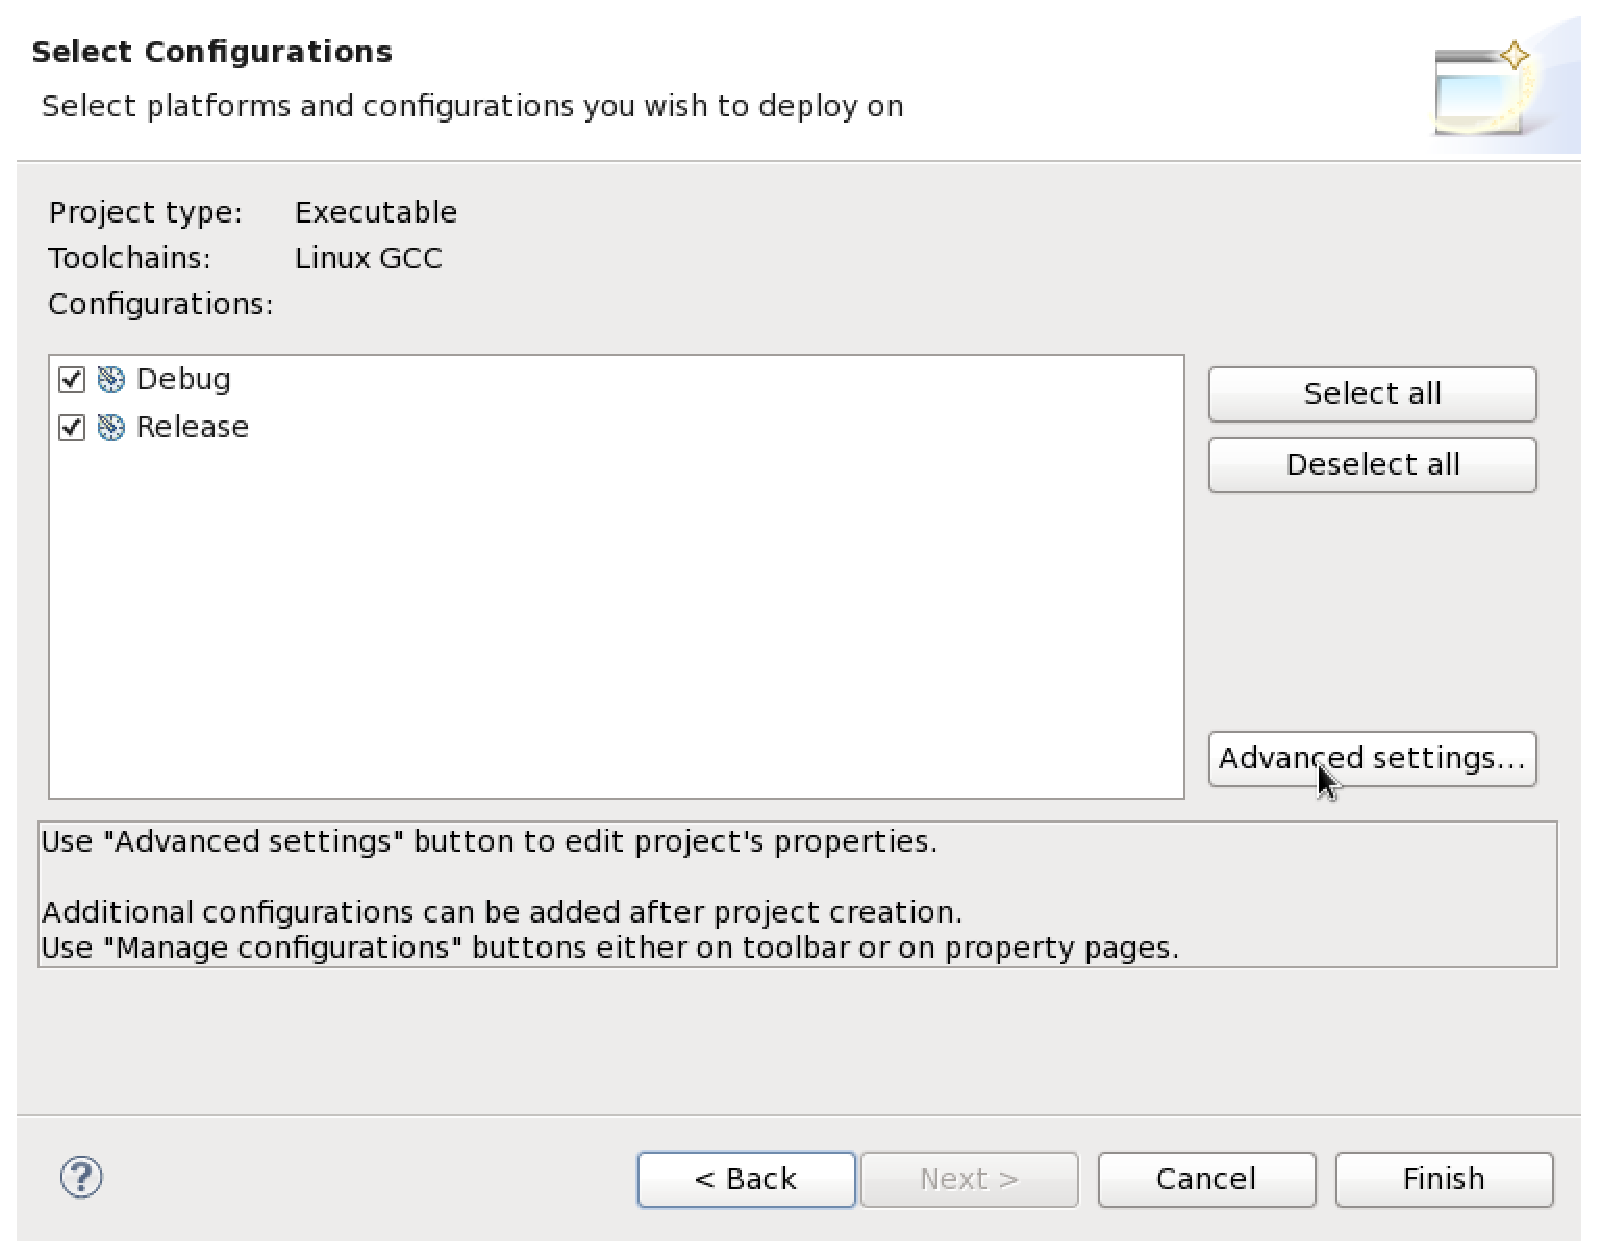
\includegraphics[width=67mm, keepaspectratio]{figures/eps/conf.eps}\hspace{1cm}
	\caption{Új Eclipse projekt létrehozása} 
	\label{fig:newproj}
	\end{figure}

\subsection{Compiler beállítása}
	A létrehozott projektre jobb gombbal kattíntva a tulajdonságára kattintva
	állíthatjuk be a fordítót a képnek \ref{fig:compiler} megfelelően.
	A beállítások kiterjednek a GNU-C99 nyelv szerinti fordításra és a korábbi
	\ref{sect:sdk} részben telepített SDK-ban található include mappa beállítására. 
	\begin{figure}[H]
	\centering
	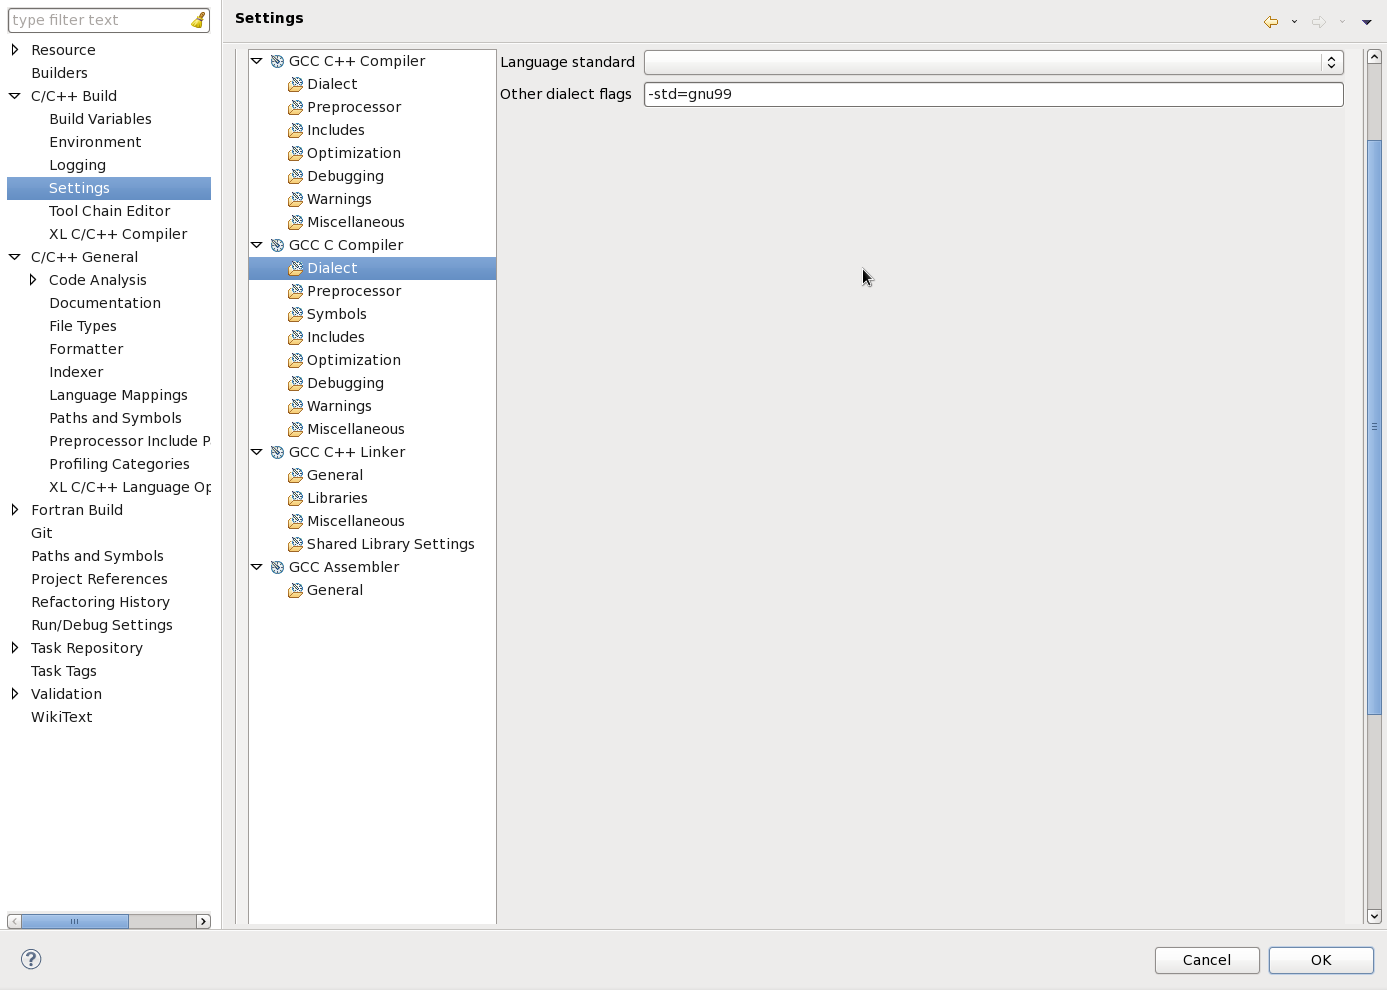
\includegraphics[width=67mm, keepaspectratio]{figures/eps/lang.eps}\hspace{1cm}
	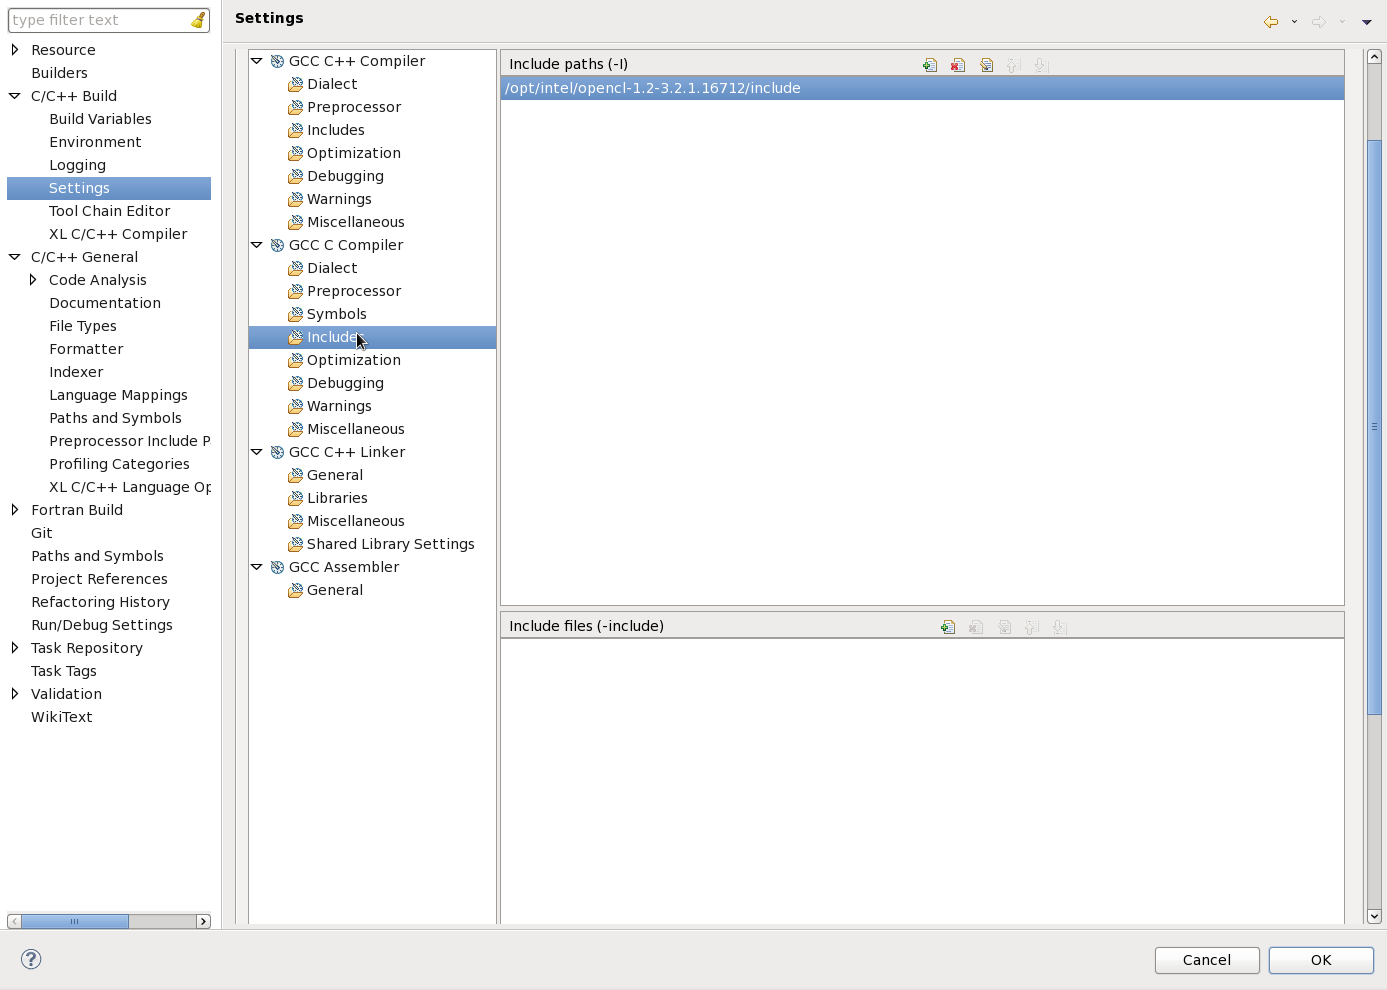
\includegraphics[width=67mm, keepaspectratio]{figures/eps/include.eps}\\\vspace{5mm}
	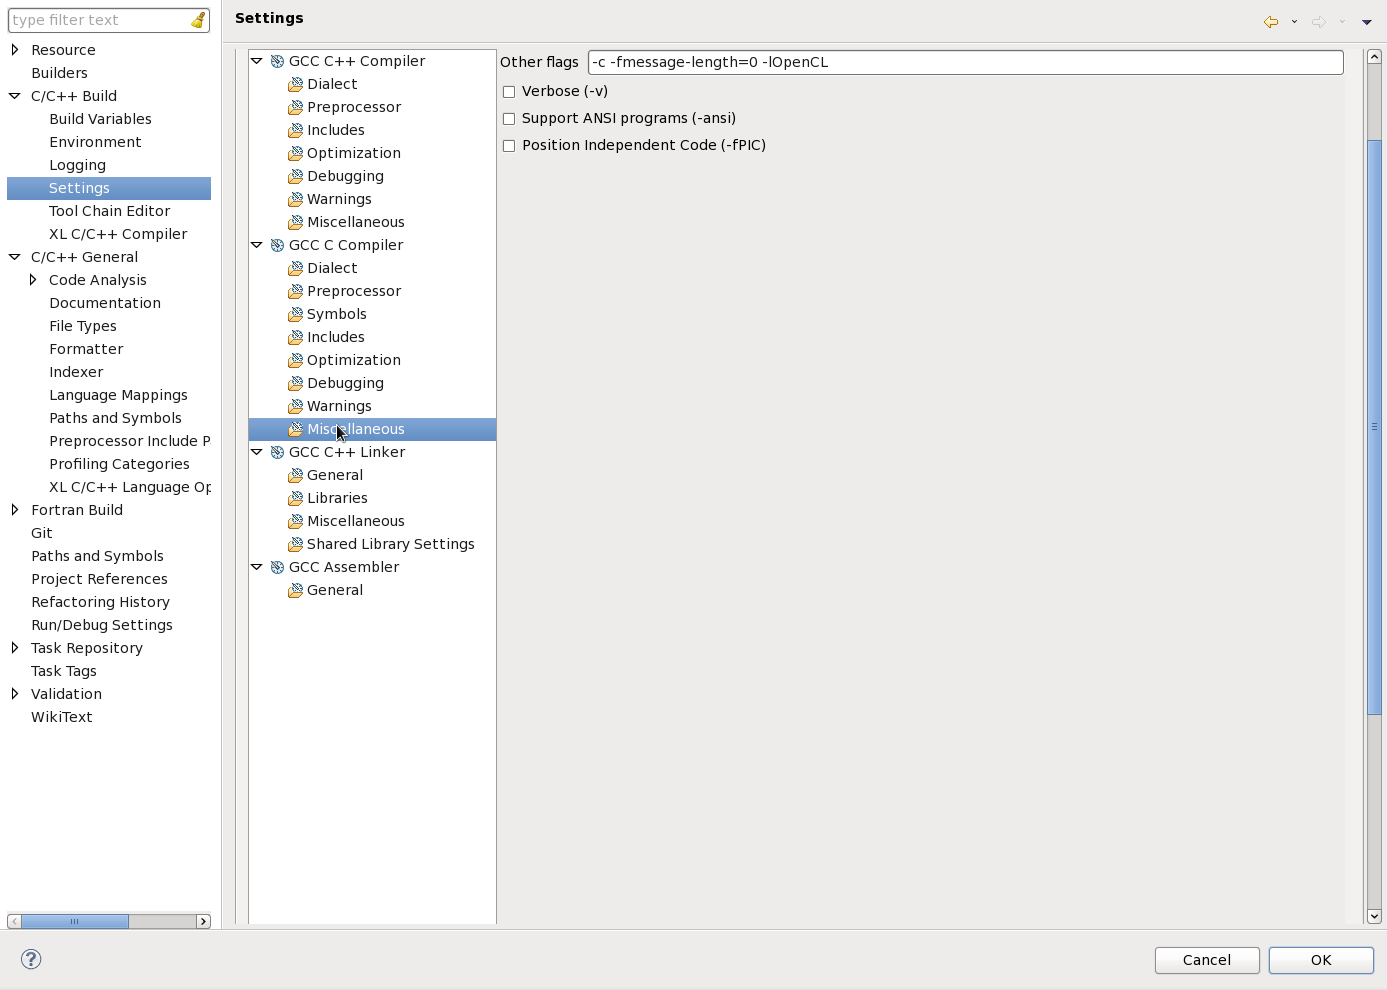
\includegraphics[width=67mm, keepaspectratio]{figures/eps/misc.eps}
	\caption{Compiler beállításai} 
	\label{fig:compiler}
	\end{figure}

\subsection{Linker beállítása}
	A linkert a \ref{fig:linker} ábra szerint állítjuk be.
	\begin{figure}[H]
	\centering
	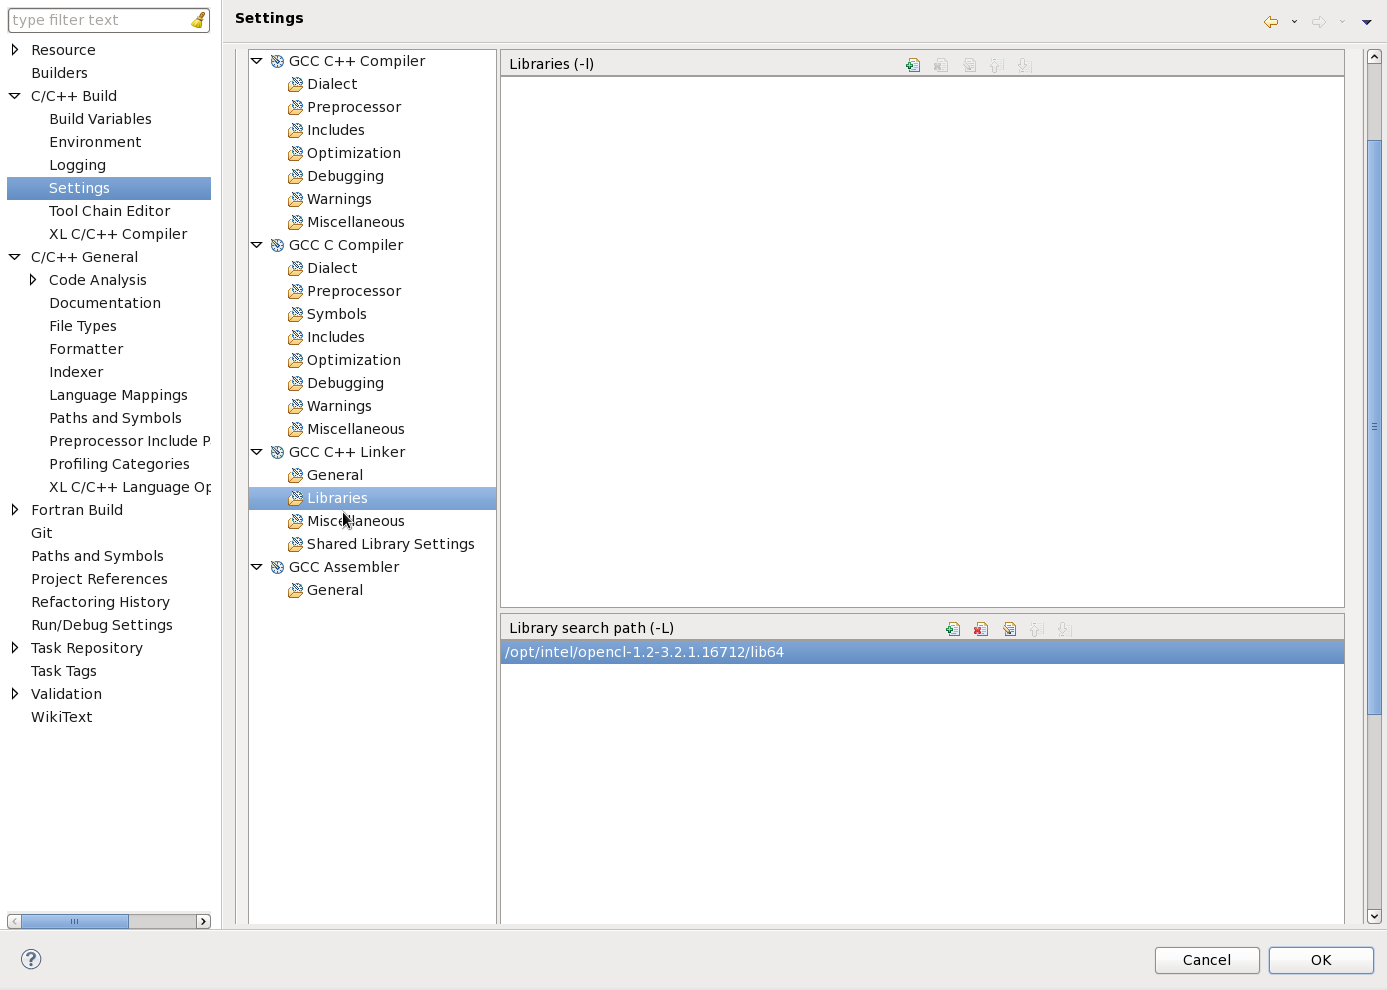
\includegraphics[width=67mm, keepaspectratio]{figures/eps/link.eps}\hspace{1cm}
	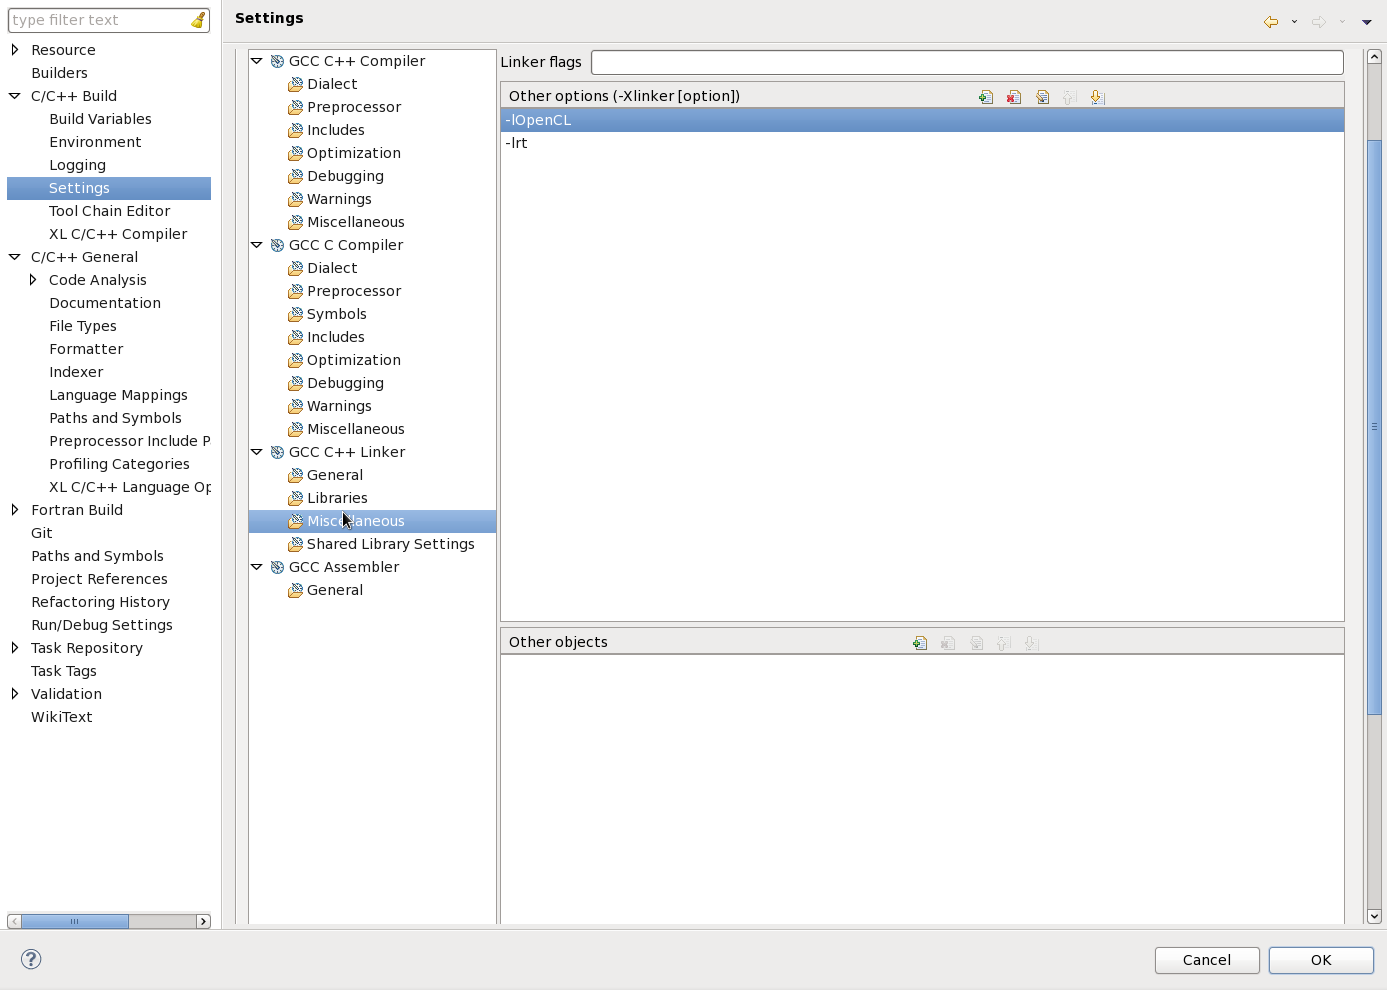
\includegraphics[width=67mm, keepaspectratio]{figures/eps/link_misc.eps}\\\vspace{5mm}
	\caption{Linker beállításai} 
	\label{fig:linker}
	\end{figure}

